\documentclass[11pt,a4paper]{article}
\usepackage[utf8]{inputenc}
\usepackage[T1]{fontenc}
\usepackage{amsmath}
\usepackage{amsfonts}
\usepackage{amssymb}
\usepackage{graphicx}
\usepackage{setspace}
\usepackage[left=2.5cm,right=2.5cm,top=2.5cm,bottom=2.5cm]{geometry}
\usepackage{float}
\usepackage[font=small,labelfont=bf]{caption}
\linespread{1.5}
\graphicspath{{./images}}

\setlength{\abovecaptionskip}{5pt}
\setlength{\belowcaptionskip}{0pt}

\title{Research Proposal: Precision Manipulation in Robotic Upper Limbs through Multi-Modal Sensing}
\author{Zilin Chen, PHD Proposal in Dept.\;of ECE, HKUST}
\date{}

\begin{document}

\maketitle

\section{Introduction}
The development of dexterous robotic manipulation remains a fundamental challenge in robotics research. While significant progress has been made in visual perception for grasping, the integration of tactile and force feedback for precision manipulation of novel objects remains underdeveloped~\cite{billard2019trends}. This research proposal aims to address the gap in robotic manipulation by developing novel control strategies that leverage multi-modal force sensing to enable \textbf{precise manipulation} of various unknown objects in unstructured environments.\\
Human manipulation capabilities far exceed current robotic systems, particularly in handling objects with varying material properties, shapes, and weights~\cite{chen2023bi}. This research will explore how advanced force sensing and control algorithms can bridge this gap, enabling robots to perform delicate manipulation tasks with \textbf{human-like proficiency}.

\section{Literature Review}
Walking has become a basic skill for humanoid robots, with researchers employing various methods to teach it. Ilija Radosavovic used reinforcement learning to enable humanoid robots to walk on several basic terrains~\cite{RL_Walking}. Scott Kuindersma improved the LQR controller to allow the Atlas robot to perform complex tasks such as dynamic walking, running, and jumping in unstructured environments~\cite{kuindersma2016optimization}. Similarly, Koolen Twan enabled Atlas to walk on uneven terrain and perform basic operations by solving a quadratic program at each control step~\cite{Atlas2}.\\
However, many researchers have also noted that robotic upper limbs—particularly achieving \textbf{human-level dexterity} in the hands—remain an unresolved challenge~\cite{10415857}. Gianpaolo Gulletta summarized the current research directions on upper limb motion of humanoid robots, pointing out that most current research focuses on single-arm reaching motion and lacks attention to dual-arm collaboration and complex manipulation tasks~\cite{robotics9040102}. He also stated that 51.85\% of studies generate trajectories by imitating human motion data rather than designing a reasonable controller and planner.
\begin{figure}[H]
    \centering
    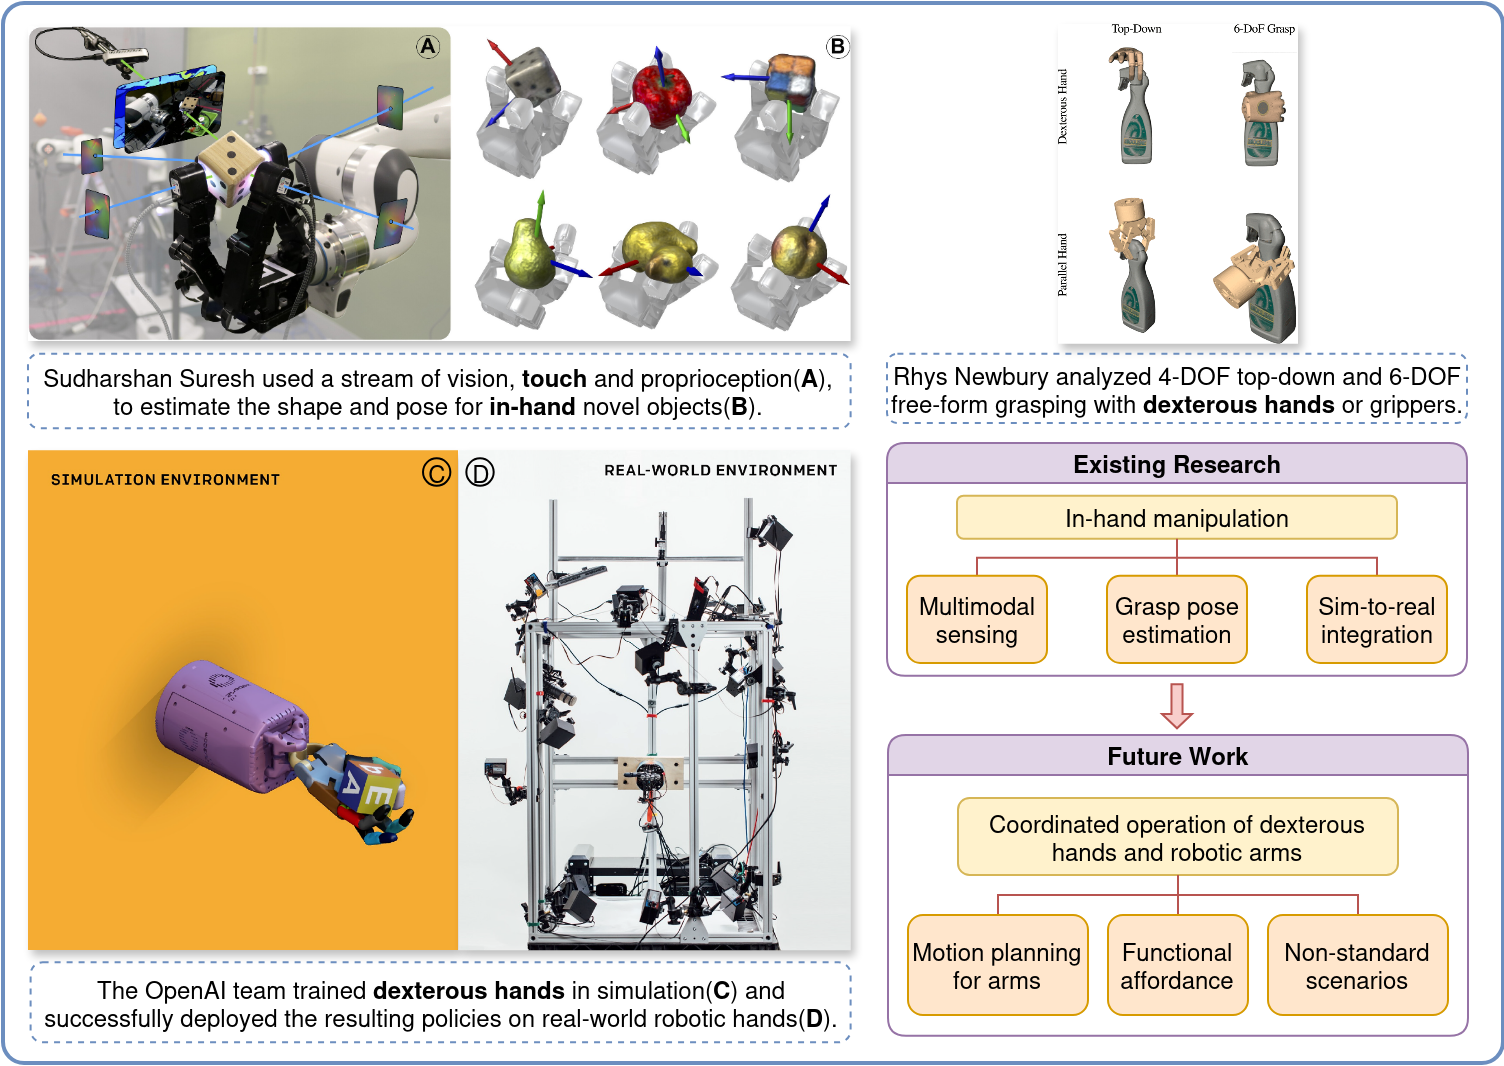
\includegraphics[width = \textwidth]{Inhand.png}
    \caption{{In-hand Existing Research\cite{suresh2024neuralfeels}\cite{newbury2023deep}\cite{andrychowicz2020learning}}}\label{inhand-fig}
\end{figure}
\noindent
Existing research on precise hand manipulation in humanoid robots mainly focuses on \textbf{in-hand} tasks, with limited work on coordinated operation of dexterous hands and robotic arms. For instance, Hanaa Yousef's review emphasizes local hand motion planning, where arm-hand coordination primarily assists hand repositioning rather than enabling more complex movements~\cite{yousef2011tactile}. Similarly, Sudharshan Suresh highlighted that achieving human-level dexterous manipulation requires understanding spatial relationships through multimodal perception, such as vision and touch. He used tactile sensing to complement visual input, but his work was still confined to in-hand manipulation without integration with the robotic arm~\cite{suresh2024neuralfeels}. Rhys Newbury and other scholars conducted a systematic review of 85 relevant papers from the past decade, highlighting future directions for grasping research. These include studying grasping in more complex environments (such as inside cabinets or in human-robot collaborative settings), integrating multimodal perception (such as tactile and force sensing), and viewing grasping as part of an overall manipulation process rather than as an isolated task~\cite{newbury2023deep}. Furthermore, he emphasized the need to consider the \textbf{functional affordance} of robotic arms—that is, not only focusing on grasp stability, but also accounting for post-grasp task requirements (e.g., when handing over scissors, one should hold them by the blades). The OpenAI team employed reinforcement learning to train policies for dexterous in-hand manipulation in simulation and successfully transferred them to a real robotic hand. Their work provides a highly feasible direction for my research, offering a reproducible framework and methodology for sim-to-real transfer. However, they relied solely on visual sensing and focused exclusively on in-hand manipulation~\cite{andrychowicz2020learning}.\\
Therefore, it is essential to develop humanoid robot upper limbs equipped with dexterous hands and robotic arms that can work in coordination, featuring multimodal perception to accurately understand and execute tasks. Among these capabilities, achieving robust multimodal perception remains a pressing challenge to be addressed. Many researchers have developed various skin-based force sensors. For example, Van Duong and Lac proposed and validated a large-scale vision-based tactile sensing system that can infer contact force and force distribution, enabling large-scale tactile perception~\cite{van2020large}. Xiong Yang also proposed a multi-layered soft tactile sensing unit called F³T, which solves the challenge of simultaneously sensing three-dimensional force (normal force and omnidirectional tangential force) and temperature in complex environments while achieving signal decoupling~\cite{YANG2025}.\\
In summary, although humanoid robots are currently a hot research topic and among the areas attracting the most capital investment, research on gait planning for humanoid robots is relatively mature, while the development of upper limb coordination remains far behind that of industrial robots or collaborative robots used in standard industrial settings. Consequently, research on the motion of humanoid robot upper limbs still holds significant untapped potential. Existing sensing technologies—particularly force sensing—can effectively support precise motion control of humanoid robot upper limbs and dexterous hands. Therefore, I aim to develop corresponding robot controllers based on these sensors to \textbf{greatly enhance the flexibility} of humanoid robot upper limbs and meet the demands of more non-standard scenarios.

\section{Research Objectives}
The overarching goal of my research is to advance the \textbf{dexterity, adaptability, and intelligence} of robotic hands by tightly integrating high-fidelity sensing, feedback-driven control, and data-driven learning. Specifically, the objectives are:

\begin{enumerate}
\item Design of high-resolution, multi-axis force sensing in robotic hands to capture rich, real-time interaction data during manipulation.
\item Development of sensor-fusion control algorithms combining force and visual feedback for adaptive, stable, and accurate grasping.
\item Creation of learning-based frameworks for generalizable manipulation across diverse objects, enabling handling of unknown items with minimal prior knowledge.
\item Experimental validation on physical robots to verify robustness, efficiency, and real-world performance of the proposed methods.
\end{enumerate}

\begin{figure}[H]
    \centering
    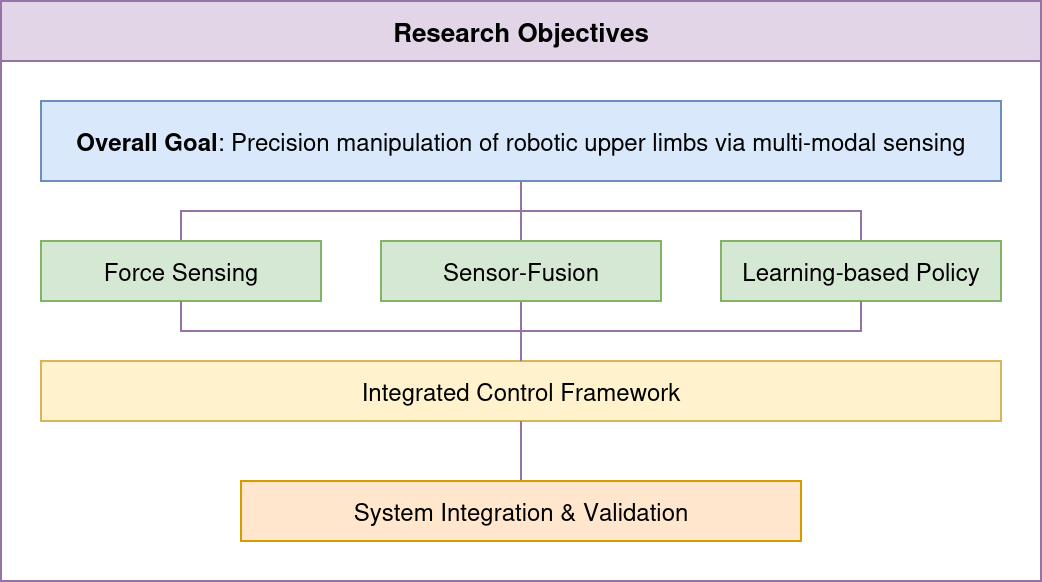
\includegraphics[width = 0.8\textwidth]{Research_Objectives.png}
    \caption{Research Framework Diagram}
\end{figure}

\section{Methodology}
The proposed research will follow a systematic approach that combines modeling, simulation, learning-based policy development, and real-world system integration. The methodology is structured into three major phases:

\subsection{Modeling and Simulation Studies}
The research begins with developing accurate kinematic and dynamic models of the robotic hand and arm. Force-sensing data will be used to analyze contact interactions during grasping. Physics-based simulations will study grasp stability, contact force distribution, and object discrimination, guiding the design of control strategies and identifying critical sensing modalities for high-precision manipulation.

\subsection{Learning-Based Grasp Policy Development}
Learning-based methods will be employed alongside modeling to achieve robust and generalizable manipulation. Reinforcement learning will train grasping policies in simulation, enabling the robot to handle diverse objects of varying sizes, shapes, and material properties. Domain adaptation techniques will transfer learned policies to the physical system, while online learning will allow continuous performance refinement during real-world tasks.

\subsection{System Integration and Experimental Validation}
The developed sensing, control, and learning components will be integrated into a complete robotic platform. The multi-fingered hand, robotic arm, and multimodal perception system will form a unified testbed. Comprehensive experiments will validate the proposed methods, benchmarking grasp success rates, force modulation accuracy, and adaptability against state-of-the-art robotic manipulation frameworks.

\section{Timeline}

\begin{itemize}
    \item \textbf{Year 1}: Conduct an in-depth literature review to identify current challenges in tactile sensing, force control, and learning-based manipulation. Establish a robotic hardware platform by integrating the multi-fingered hand, robotic arm, and vision system. Implement the data acquisition and processing infrastructure. Perform preliminary experiments to verify sensing accuracy, system calibration, and baseline performance.
    
    \item \textbf{Year 2}: Develop the core control and learning algorithms, including hybrid control strategies and reinforcement learning policies. Perform extensive simulation studies to validate stability, safety, and adaptability. Collect sufficient experimental data in both simulation and physical environment. Begin domain adaptation research to prepare for transferring learned policies from simulation to physical hardware.
    
    \item \textbf{Year 3}: Deploy the developed algorithms onto the real robotic platform. Conduct extensive experimental validation across a wide range of manipulation tasks and object types. Benchmark performance against state-of-the-art methods using quantitative metrics such as grasp success rate, force modulation accuracy, and real-time responsiveness.

    \item \textbf{Year 4}: Refine the integrated system based on experimental findings. Finalize the dissertation with comprehensive documentation of methodologies, results, and theoretical insights. Complete thesis defense and disseminate research outcomes to the broader robotics community.
\end{itemize}

\section{Conclusion}
This research proposal outlines a comprehensive approach to advancing robotic manipulation capabilities through innovative use of force sensing technology. By combining rigorous theoretical development with practical implementation, this work aims to significantly advance the state of the art in robotic manipulation and contribute to the broader field of embodied intelligence. The proposed research aligns perfectly with Professor Shen's focus on embodied intelligence and \textbf{precision upper limb control}, offering exciting opportunities for fundamental advances with practical applications.

\vspace{100pt}

\bibliographystyle{IEEEtran}
\bibliography{references}

\end{document}